\documentclass[journal,compsoc]{IEEEtran}
\usepackage{booktabs,amsmath,graphicx,hyperref}
\hypersetup{hidelinks}
\title{EvoAgent: Evidence Checks and Controlled Evolution for Pull Request Review}
\author{EvoAgent Project Team\\Tianyi Jiang (72612066), Jianyu Zhou (72610417), Jiayu Zhu (72610189),\\ Siye Tu (72610036), Xinyu Zhang (72610510), and Jiexuan Shen (72610012)}
\begin{document}
\maketitle
\begin{abstract}
EvoAgent assists developers reviewing pull requests by linking reported findings to changed lines. The project begins with a single model baseline and introduces fixed role collaboration, bounded tools, recovery checkpoints, repository feedback and controlled skill evolution. The final snapshot adds batch coverage and report confirmation. Its local regression suite passed 84 tests. On a 100-case controlled offline comparison, evolving the skill did not improve held-out F1 over the matched workflow. A separate 130-case prompt replay improved synthetic holdout F1 from 66.67\% to 100\%, with production activation rejected by the data provenance check. A live pilot on a public documentation pull request completed in batched mode in 27.415 seconds using 9,262 recorded tokens. The legacy path exceeded its execution budget on the same diff. The evidence supports functional acceptance of the tested behavior and quantifies limitations of the offline comparison. It leaves comparative accuracy on representative real pull requests open.
\end{abstract}
\begin{IEEEkeywords}
Code review, pull requests, software testing, evidence validation, software evolution.
\end{IEEEkeywords}

\section{INTRODUCTION}
Pull-request review asks developers to inspect changed code under limited time and context. A reviewer must separate actionable defects from plausible but unsupported claims, identify the changed line, and explain how the issue could be fixed and tested. EvoAgent addresses this workflow with a review assistant that receives a unified diff and returns structured findings tied to observable diff evidence. Its intended user is a developer or development team reviewing a pull request before merging it.

The bounded problem is to increase the usefulness and traceability of review findings without granting the assistant unrestricted repository authority. The project studies whether specialist roles, controlled context selection, and feedback-based skill changes can improve on simpler baselines. It does not claim that an offline synthetic result measures performance on all real repositories.

The engineering contribution is the integration of three checks that operate at different stages. The runtime constrains what evidence a reviewer can access. The publication gate checks the location and quotation of each candidate finding. The evolution gate determines whether a candidate configuration is eligible for deployment. The tests and replay studies assess these checks at the corresponding interfaces.

\section{RELATED WORK AND BACKGROUND}
Earlier neural approaches cast parts of review as sequence-to-sequence transformation. Tufano et al. studied two tasks: revising code before review to anticipate likely reviewer changes, and applying a reviewer’s natural-language comment to submitted code. Their pre-trained T5 approach improved on earlier deep-learning models and was tested on a larger, more realistic review dataset [1]. These tasks differ from EvoAgent’s primary task: producing structured findings on a pull-request diff. In particular, a code revision can be useful without being a review comment tied to an exact added line; a comment-only output needs a separate check that its claimed location is present in the diff.

Li et al. introduced CodeReviewer, a model pre-trained on code changes and reviews from open-source projects in nine programming languages. It uses review-specific pre-training tasks and evaluates code-change quality estimation, review-comment generation, and code refinement [2]. CodeReviewer establishes that training on review data can support several distinct activities. EvoAgent instead emphasizes the operational path around a generated finding: parsing a unified diff, selecting bounded context, and checking path, added-line location, and cited evidence before publication. This is a difference in system emphasis and output validation, not evidence that EvoAgent has higher review accuracy. The two systems would need a shared dataset and matching metrics for such a claim.

Multi-agent review is especially close to EvoAgent’s collaborative workflow. Tang et al. proposed CodeAgent, in which communicating agents and a supervisory QA-Checker address code-change and commit-message consistency, vulnerability introduction, style compliance, and code revision [3]. EvoAgent likewise separates lead, specialist, critic, and synthesis responsibilities. Its implementation additionally exposes role-scoped read-only tools, resource budgets, checkpoints, and explicit diff-evidence and skill-activation gates. These design choices target traceability and bounded execution. CodeAgent’s published task results cannot be compared numerically with EvoAgent’s controlled offline fixtures because the tasks, datasets, model execution, and outcome measures differ. A common real-PR evaluation would be needed to determine whether these choices improve practical review quality.

Evaluation design is another relevant strand of work. Zeng et al. introduced SWR-Bench with 1,000 manually verified GitHub pull requests and full project context, aiming to evaluate review-comment generation at PR level [4]. Its design highlights the gap between isolated or synthetic cases and reviews conducted in a repository. EvoAgent’s current V5 evidence consists of automated acceptance tests and two labelled offline replay suites. Those suites can verify deterministic behavior and compare controlled arms, but they do not estimate performance on SWR-Bench or other real-PR populations. A later comparison should freeze the task, ground truth, baselines, model settings, and precision/recall criteria before running EvoAgent and competing tools on the same cases.

Together, these studies cover learned code transformation [1], review-specific pre-training [2], collaborative agents [3], and realistic PR-level measurement [4]. EvoAgent’s proposed contribution is the engineering combination of collaboration with explicit evidence, authority, and activation gates. The current report treats that as a design claim; its comparative effectiveness remains an empirical question for a shared benchmark.

\subsection{Review Data and Evidence}
A unified diff records additions and context for changed files. EvoAgent parses this representation and checks whether each proposed finding points to a valid added line with matching evidence. This does not prove the semantic correctness of a finding, but it prevents a class of ungrounded location claims. Context selection and repository memory provide supporting material while preserving boundaries on size, scope, and trust.

\section{REQUIREMENTS AND ARCHITECTURE}
The central functional requirement is to accept a pull request or diff, run a review, and return a report with actionable findings and test suggestions. Later increments add collaborative roles, bounded tools, adaptive context and memory, and controlled skill evolution. The architecture separates HTTP and GitHub integration, the review service, task storage, agent runtime, context and memory selection, finding gates, and evaluation harnesses.

\subsection{Security and Isolation}
The first non-functional requirement is security and isolation. Repository-derived text is treated as untrusted input; role-scoped tool permissions and parameter schemas constrain tool use. Authentication and repository or tenant boundaries protect stored state. This design aims to prevent a review of one repository from reading another repository’s memory or expanding an agent’s authority through its prompt. Acceptance tests should verify cross-tenant access denial and blocked out-of-role tool calls.

\subsection{Reliability and Recoverability}
The second non-functional requirement is reliability. Runtime budgets limit steps, calls, tokens, and elapsed time; checkpoints record completed work so interrupted reviews can resume without rerunning completed nodes. Task states distinguish completion, failure, pause, and cancellation. These choices make failures inspectable and bound resource consumption. Acceptance tests should verify budget enforcement, checkpoint reuse, and explicit terminal states.

\subsection{Review Workflow}
The baseline version uses a single model call. The collaborative increment adds a lead, specialist workers, critic, and final synthesis. Tool-assisted review limits agents to registered read-only operations over bounded diff context. Adaptive review chooses context according to risk, recalls repository-specific feedback, and selects declarative role-scoped skills. Controlled evolution evaluates proposed skill changes against validation and holdout cases before activation; rollback remains available.


\section{Software Process}
The course asks for three Sprints, weekly discussions and a whole-project burndown. We grouped repository activity using the course periods and the version increments visible within those periods. Sprint 1 covers V1. Sprint 2 covers V2 and V3. Sprint 3 covers V4, V5 and the separately selected final snapshot. Weekly development was scoped to Weeks 2--12. The team closes Sprint 3 on 30 November, and Week 13 remains the course window for final delivery. The 27 November Sprint Review and Retrospective remained scheduled when this report was updated on 24 November.

\begin{table*}[t]
\caption{Team-supplied Sprint calendar and repository increments in 2026}
\centering
\begin{tabular}{lllll}
\toprule
Sprint & Team period & Planning & Review and Retrospective & Repository increments \\ \midrule
1 & 7 September--4 October & 7 September & 2 October & V1 \\
2 & 12 October--8 November & 12 October & 6 November & V2 and V3 \\
3 & 9--30 November & 9 November & 27 November (scheduled) & V4, V5 and final delivery \\ \bottomrule
\end{tabular}
\end{table*}

The team confirmed that all six members attended the meetings already held. The discussion accounts below reconstruct technical matters from backlog, repository and test evidence. They do not establish the precise words used in meetings, the adoption of every retrospective action or the signature of an accepting reviewer. The weekly Discussion calendar lists Fridays at AC5-302, 15:00--18:00. Its 27 November and 4 December entries were future appointments at the time of writing.

\subsection{Sprint 1: Establishing a usable baseline}
Sprint 1 focused on the single-call path from a pull request to a saved review report. Planning covered configuration, GitHub intake, asynchronous state, structured findings, a task view and initial verification [8]. Source and tests appeared on 13 September, followed by a restored snapshot and backlog on 22 September. By the 2 October Review the repository contained the intake, view and parsing evidence for that increment. The archived V1 regression later reported two passing tests. This is evidence for the tested behavior in the recovered snapshot. A live historical acceptance still requires a dated run and reviewer record.

The technical review of this increment emphasizes the seams between the service, the provider and the report. A small system could make these boundaries inspectable before the role workflow complicated execution. The documented improvement for subsequent work was to keep the visible output contract while adding specialist proposals, independent Critic checks and report evidence. We retained V1 as an implementation baseline. Results from an experiment using a different legacy path are identified separately in the Evaluation section.

\paragraph{Review discussion reconstructed from the 2 October evidence.}
The technical discussion record follows V1 from configuration and PR URL validation to diff retrieval, the background task, one model call and report display. The later two-test regression supports parsing and normalization. A positive run with a valid URL and a rejection check with an invalid URL were identified as follow-up acceptance items. For the next increment, the record proposes retaining a fixed input diff and adding independent findings checks. This preserves a baseline for evaluating the move to a multi-role workflow. The team confirmed attendance. The available artifacts do not establish a formal acceptance decision.

\subsection{Sprint 2: Collaboration and bounded execution}
V2 introduced fixed role collaboration, path and added-line checks, role-level accounting, and a view of delivery state [9]. Its backlog and source were uploaded on 18 October. The 6 November Review record can therefore discuss V2 as repository evidence. V3 source was uploaded on 7 November, within the Sprint period ending on 8 November. We record V3 as Sprint-end follow-up. The upload date alone gives no basis for stating that V3 was demonstrated at the preceding Review.

V3 developed the transition from a fixed workflow to bounded tool inspection, budget checks, checkpoints and cancellation [10]. It also strengthened the rule that final synthesis must preserve findings already checked by the Critic. The retrospective technical account identifies the additional model calls, state transitions and provider failures introduced by collaboration. A later regression evaluation recorded 33 passing tests for the local V2 snapshot and 54 for V3. Those runs document later verification. They do not serve as sign-offs for the 6 November meeting.

\paragraph{Review discussion reconstructed from the 6 November evidence.}
The V2 evidence supports separate inspection of role traces, report findings and GitHub comment delivery. The reconstructed discussion considers whether a report should admit findings with a wrong path, a non-added line, mismatched quoted evidence or duplicate evidence. It also separates successful report generation from successful posting. The carry-forward items are to compare the single-call and collaborative workflows on a frozen diff and to capture completed work before interruption. The 7 November V3 upload records Sprint-end progress on those runtime controls. The later V2 and V3 regressions, with 33 and 54 passing tests respectively, support the released snapshots. They do not establish which build was demonstrated on 6 November.

\subsection{Sprint 3: Adaptive context, evolution and release}
Planning on 9 November assigned work on bounded risk context, scoped feedback, skills, evaluation, recovery and release. The V4 restored snapshot was uploaded on 21 November, and V5 was uploaded on 23 November at commit \texttt{faf93a1}. The separate selected delivery branch contains commit \texttt{b9a63e3}, uploaded on 21 November. This chronology leaves V5 as a development reference and the selected branch as the release identity. We do not assign a version number to the selected branch. The restored V4 and V5 packages contain shared infrastructure. Their stated version scope determines which features are attributed to each increment.

The 27 November Review and Retrospective were planned to verify the selected source, discuss the staged evaluation, inspect batch coverage and recovery, and confirm outstanding delivery work. The technical evidence prepared for those discussions includes 70 passing V4 tests after maintenance, 70 for V5 and 84 for the packaged final source. The offline study rejected an evolved skill candidate that did not improve the matched holdout. A separate prompt replay showed a numerical gain on synthetic fixtures, with production activation blocked by the provenance gate. The live pilot recorded one completed batched run and one legacy budget failure. A future meeting outcome is deliberately left open.

\paragraph{27 November Review and Retrospective agenda.}
Tianyi Jiang and Xinyu Zhang are assigned to present the V4 context limits, isolation checks and corrected regression run. Jianyu Zhou and Siye Tu are assigned to explain the lack of holdout F1 gain in the 100-case Skill comparison and the separate 130-case prompt replay that passed the numeric threshold but failed the production provenance gate. Jiayu Zhu is assigned to demonstrate partial coverage, resume and revision confirmation using the deterministic trace. Jiexuan Shen is assigned to reconcile the pinned release, its 84-test evidence and the incomplete legacy pilot run before the team decides on acceptance. The agenda identifies proposed presenters. Attendance, adopted actions and sign-off will be recorded after the meeting.

\section{EVALUATION}
\subsection{Automated Acceptance Checks}
The V5 code passed 70 automated tests after restoring the two fixture datasets from another available project copy. The suite exercises review parsing, evidence gates, runtime budgets and checkpoints, memory isolation, skill evolution, API and service behavior, and production-oriented features. Python compilation and JavaScript syntax checks also passed. A passing test suite establishes expected behavior for covered scenarios; it is not an accuracy estimate on live developer pull requests.

\subsection{Controlled Comparison}
The first offline dataset has 100 synthetic cases [6]. For the controlled five-arm comparison, cases are split by repository into 60 train, 20 validation, and 20 holdout examples. The execution mode is explicitly “controlled-offline-no-llm”: it evaluates deterministic rules, orchestration accounting, and skill selection without invoking a real language model. In the full controlled set, the single reviewer arm yielded F1 71.43\%, the scanner arm F1 82.50\%, and the full agentic arm F1 90.41\%. These aggregate values should not be presented as real-LLM performance. On the hidden holdout, the critic, multi-agent, and evolved-skill comparisons produced no F1 gain over their matched baselines. The skill-evolution candidate was rejected at validation and activation remained blocked.

\subsection{Prompt-Evolution Replay}
A separate 130-case synthetic replay used 104 validation and 26 holdout cases from ten fixture repositories [7]. Feedback from 32 validation misses generated a candidate prompt version. In the controlled replay, both validation and holdout F1 increased from 66.67\% to 100\%. The quantitative gate passed, but the production provenance gate failed and production activation was blocked because the cases were offline fixtures. This result supports the behavior of the replay and gate, not generalization to real GitHub pull requests.

\subsection{Threats to Validity}
The present datasets are labelled offline fixtures with no public PR URLs. They are useful for deterministic regression and acceptance scenarios but may underrepresent project-specific coding conventions, long diffs, ambiguous defects, and imperfect human labels. The two experiments also ask different questions: one evaluates controlled role and skill arms without a real LLM, while the other demonstrates a prompt-version replay. Their scores should not be pooled or used to claim that the same skill improvement appears in both settings.

\section{Final Snapshot and Regression}
\begin{table}[h]
\caption{Regression tests on the available local snapshots}
\centering
\begin{tabular}{lrl}
\toprule
Snapshot & Tests & Result \\ \midrule
V1 & 2 & Pass \\
V2 & 33 & Pass \\
V3 & 54 & Pass \\
V4 before maintenance & 70 & 1 failure and 5 errors \\
V4 after maintenance & 70 & Pass \\
V5 & 70 & Pass \\
Final & 84 & Pass \\ \bottomrule
\end{tabular}
\end{table}
The restored V4 test suite referenced two missing fixture files. We restored the shared offline fixtures from the available V5 snapshot. One additional test checked a Python assignment as literal text, causing it to fail when the expression used single quotes. We changed the assertion to compare the syntax tree of the expected assignment. The test continues to check the supported rule set and preserve unsupported statements. The complete V4 suite passed after both changes. Previous and current logs are provided so that the original regression and the maintenance result remain distinguishable.

The final snapshot divides a larger change into batches and records completed and outstanding units. A report shows coverage as well as findings. When a task pauses within its budget, the service retains completed work. Resume processes outstanding units and preserves locations on the original diff. Confirmation of a report requires a specific revision so a reviewer can verify the exact text accepted. An incomplete or inconsistent change must retain the appropriate coverage status. The integration tests exercise long lines, deletions, inconsistent hunks, pause and resume, and repeated confirmation.

\subsection{Architecture and acceptance rationale}
The isolation requirement applies to both evidence access and historical feedback. We bound tool inputs and select from registered operations, and keep feedback scoped to its repository and tenant. This limits cross-repository contamination even when candidate text includes irrelevant instructions. Acceptance covers denied access and memory isolation. An additional deployment acceptance step should validate the expected configuration in the submission environment.

The recoverability requirement limits repeated work after interruptions. The runtime tracks completed steps and enforces explicit budgets. A resumed job must preserve those checkpoints and may retry only the outstanding stage. Acceptance checks the paused state, the preserved partial report and the final recorded revision. Timeout and partial coverage both remain visible to the consumer. External model availability and completion cost require empirical measurements under the actual service configuration.

\subsection{Public pull request execution pilot}
A documentation change from the public Click project (PR 88) is frozen with a diff checksum and revision metadata. The comparison uses the legacy and batched paths of the final release, separate local databases, identical model settings and review publishing disabled. It checks that the workflow can process a real diff through a configured service. The run log records each arm, duration, status and usage where available. Empty reference findings for this functional pilot do not constitute reviewer labels. The first attempts failed TLS certificate verification. A retry with the system CA bundle reached the 150-second outer deadline without a paired result. An independent model request over the same public diff succeeded in 7.511 seconds with 1,105 tokens. A subsequent retry used separate processes for both engines, MiMo v2.6 Pro and an initial token budget of 12,000. The batched engine completed one of one batches in 27.415 seconds, used 9,262 recorded tokens and produced zero findings. The legacy engine stopped at its execution budget after 45.876 seconds. Its token usage and coverage were unavailable. The pilot confirms completion on this input under the recorded settings. A single documentation change with no independent reference labels cannot support a comparative accuracy or reliability claim.


\subsection{Project burndown}
\begin{figure*}[t]
\centering
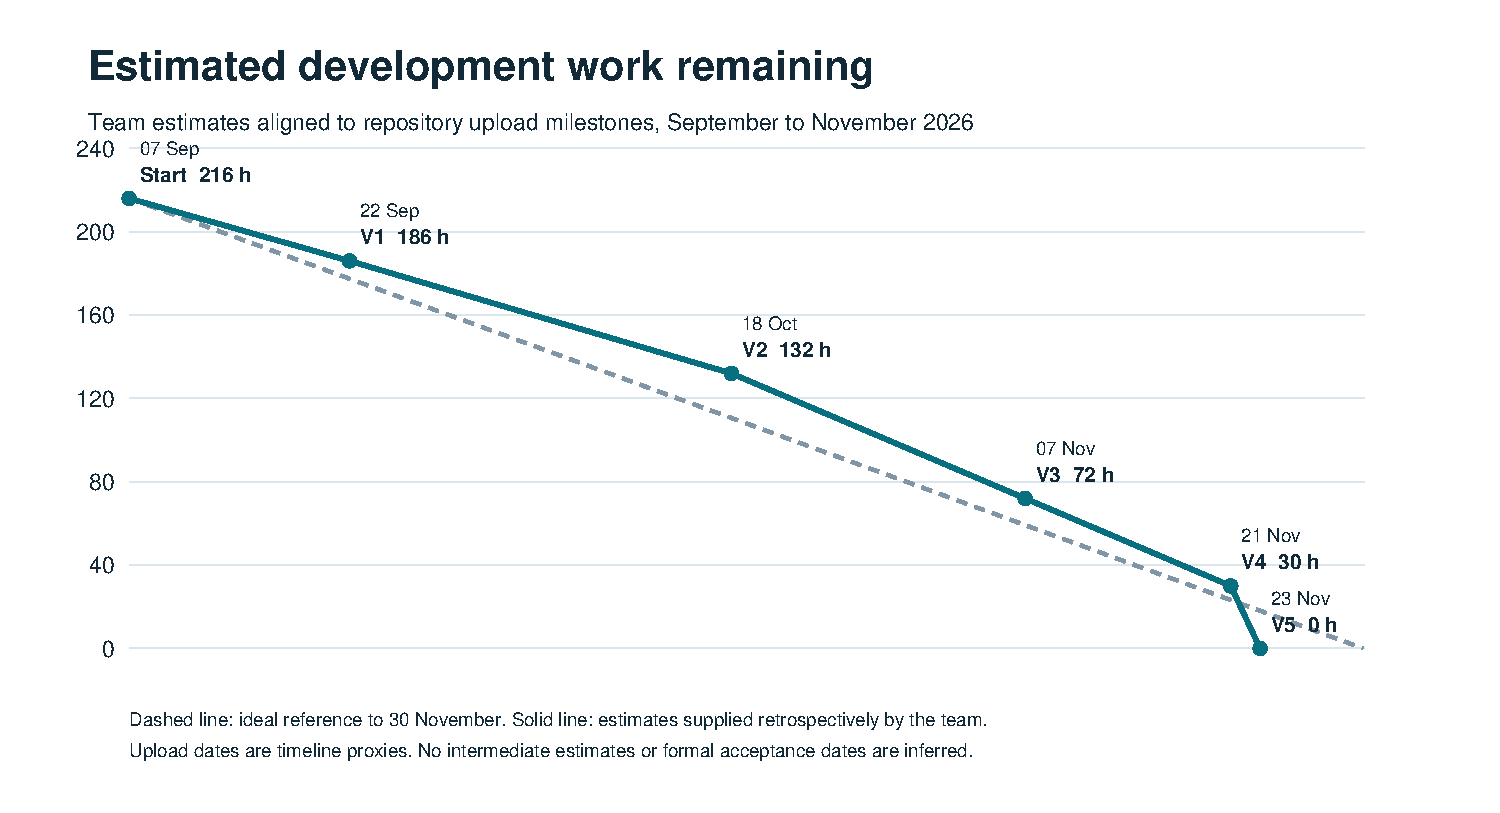
\includegraphics[width=0.87\textwidth]{EvoAgent-Milestone-Burndown.pdf}
\caption{Retrospective estimates of remaining development work at repository upload milestones. The dashed line represents the ideal reference from 7 September to the planned Sprint close on 30 November.}
\end{figure*}
The team supplied a starting estimate of 216 hours and successive remaining-work estimates of 186, 132, 72, 30 and 0 hours for V1 through V5. We position these values on the dates of the selected version uploads. The spacing therefore represents repository activity. Intermediate estimates were unavailable and the segments simply connect the reported samples. The estimate of zero applies to the team's development scope. Report completion, rehearsal, submission and other delivery work are tracked separately. The curve cannot be converted to actual labor or individual hours.

\section{Contribution Allocation}
The contribution record uses the four repository backlogs as evidence of assigned work. Task identifiers below refer to their respective backlogs. V3 packages cover planned work, including repair-related assignments. Verified implementation and test evidence identify which outcomes the report can claim. For V5 and final delivery we assign six coordination packages because the archived workbooks do not contain equivalent named assignments for those increments.

\par \textbf{Tianyi Jiang}. V1: PR metadata and diff retrieval (SB-05). V2: QA and Scrum (SB13--SB15). V3: Runtime, budgets, and checkpoint recovery (01--03). V4: Risk ranking and bounded diff context (T01--T03). V5 and final delivery assignment: Maintain release reproducibility. Verify clean setup, configured dependencies and matching source hashes.
\par \textbf{Jianyu Zhou}. V1: Runtime artifact handling and baseline model call (SB-03, SB-08). V2: Review integrity (SB06, SB09, SB12). V3: Tool contracts and read-only inspection (04--06). V4: Scoped memory, recall and expiry (T04--T06). V5 and final delivery assignment: Own evaluation reproducibility. Verify offline splits, model settings, pilot outcomes and limits on claims.
\par \textbf{Jiayu Zhu}. V1: PR URL validation (SB-04). V2: Platform integration (SB07--SB08). V3: UI, API, acceptance tests and demo (16--18). V4: Adaptive integration and release handoff (T16--T18). V5 and final delivery assignment: Own final user-flow acceptance. Walk submission, report coverage, resume and confirmation.
\par \textbf{Siye Tu}. V1: Local HTTP service and dashboard hosting (SB-02). V2: Model integration (SB02, SB04). V3: Publication evidence, untrusted input, and diff trimming (07--09). V4: Skill manifests and role selection (T07--T09). V5 and final delivery assignment: Own evolution workbench acceptance. Check candidate provenance, gate outcomes and release identity.
\par \textbf{Xinyu Zhang}. V1: Configuration and webhook deduplication (SB-01, SB-07). V2: Frontend and comparison entry (SB10--SB11). V3: Repair-policy and patch work packages (10--12). V4: Tenant isolation and tool permissions (T10--T12). V5 and final delivery assignment: Own packaged regression and access-control verification. Preserve before/after logs and rejected actions.
\par \textbf{Jiexuan Shen}. V1: Asynchronous task lifecycle (SB-06). V2: Workflow design (SB01, SB03, SB05). V3: Verification gate and reporting (13--15). V4: Task budgets, checkpoints and cancellation (T13--T15). V5 and final delivery assignment: Own final runtime and process evidence. Reconcile task states, incomplete coverage and Sprint acceptance records.

The final handoff allocates concrete outputs across the six members. Tianyi Jiang checks archive identity and clean setup. Jianyu Zhou prepares an evidence record for the offline splits, negative Skill result and paired PR run. Jiayu Zhu records the review path from submission through complete coverage and confirmation. Siye Tu documents candidate evaluation, provenance and the conditions for activation. Xinyu Zhang checks access boundaries and retains the V4 maintenance and packaged-release regression logs. Jiexuan Shen reconciles the runtime trace, partial coverage and decisions from the release Review. These are final delivery assignments. The V1--V4 task identifiers above are historical backlog ownership. Individual completion and authorship can be confirmed with the corresponding evidence and each member's statement.

Hours remain team planning estimates. Each member owns an identifiable output and can attach completed-work evidence for their contribution declaration. Biographies and personal reflections require member input.

The detailed records are maintained alongside this report. See the \href{https://github.com/Theo-sssssss/CS5351-Project/tree/6d5354a55d89e5d0cda04429d8007028f9ced160/docs/final-submission/process}{Sprint discussions and contribution traceability records}.

\section{System and Acceptance Walkthrough}
\subsection{From a pull request to a report}
A pull request review begins with a repository identity and a diff. The object being reviewed is a set of changes rather than a complete checkout. In the simplest workflow the developer supplies the diff directly. A GitHub integration can obtain it from a pull request event. The service represents the resulting work as a task, so a review has an identity and state that can be queried independently of the HTTP request that started it. This is useful for pull requests that need several model calls or exceed an interactive request duration.

The diff parser associates each changed input with a path and lines on the old and new sides. The reviewer for a task consumes a selected portion of that representation. The result is a structured candidate containing the claimed location and evidence. The publication check looks the candidate up in the original parsed diff. An unknown path, a context line where an addition was required, or a quotation inconsistent with the indicated line prevents publication. A warning can still be semantically wrong when it cites valid text. The report therefore gives the developer a stable point to inspect and explain why they accept or reject the finding.

Our baseline makes a single model call. The role workflow creates a plan, runs focused reviews and evaluates candidates with a Critic. The final summary is useful for understanding the complete result, but rewriting individual findings after critique can remove evidence or change the claim being approved. The V3 integrity change preserves findings that have already passed review and uses the final generation for the summary. Regression cases exercise valid and invalid candidate locations independently of the summary. This makes errors at the report interface easier to distinguish from failures in candidate generation.

\subsection{Flow and scope of a batch}
The larger input workflow records the units it handles and the status of each unit. A final report can point back to the corresponding locations after splitting. Acceptance checks deliberately include a long line, deletions and an inconsistent hunk. The main design concern is that a reported line remains meaningful in the original diff even if the chunk boundary changes. A malformed hunk therefore cannot count as complete merely because a model call returned a response.

The executable demonstration uses twelve file changes and a deterministic model fixture. The task pauses at the initial budget after two batches. The partial report exposes the progress and the task rejects a mismatched report revision. After the test adds budget, the service runs the remaining work. The test compares the task trace before and after resume to check that completed batches were reused. The completed report exposes full coverage and accepts a matching revision. A repeated confirmation returns the existing outcome, which is relevant when a client retries after an uncertain response. A separate tenant cannot confirm that task.

The fixture is a repeatable acceptance scenario for state changes and does not model network behavior, token billing or model reasoning. For a live pilot, we fix the PR diff and model configuration before testing both paths. We track transport failures separately from failed reviews. An offline test can pass while a service provider is unavailable. Recording both observations helps the team improve runtime behavior without attributing transport failures to the correctness of reviewer output.

\subsection{How feedback reaches production}
An accepted finding or reviewer correction can be recorded with its originating task and repository context. The design allows that information to propose a candidate change to a review skill or prompt. The old version provides a comparison target. Replay evaluates sample behavior before the version can be activated, and the service records the evaluation and provenance decisions separately. A human still controls publication and can restore a previously available version. These controls make it possible to audit whether an observed outcome came from a change in model configuration or a change in the evaluated cases.

There are three possible kinds of failure during this workflow. The candidate may score below a required threshold. The validation data may lack the source evidence required for production. The candidate may pass the applicable checks but remain unpublished while a human reviews it. Presenting these outcomes distinctly prevents an evaluation receipt from being mistaken for a deployed change. The reported offline experiments exercised the first two outcomes. The controlled skill candidate showed no benefit on the matched holdout. The prompt replay passed numerical checks on its fixture but its production activation was blocked.

\subsection{Interpreting subsequent evaluation}
A comparative review study needs an explicit definition of a matching finding. Candidate predictions can refer to the same issue with different descriptions or adjacent code locations. Human adjudication should check whether each finding identifies the same behavior and location range as the reference. Duplicates count once against the same reference issue. A prediction with valid quoted evidence can still be a false positive. An incomplete run requires a separate execution status so that failed cases do not become successful empty reviews.

For a fixed set of reviewable changes, report precision as the fraction of emitted findings matched by the adjudication and recall as the fraction of reference issues matched. Report the actual denominators and the share of reviews that completed. For clean cases, report how often a completed review produces no unsupported finding. These measures answer different questions. A conservative reviewer can appear precise while omitting important issues. A larger candidate list can appear thorough while increasing reviewer effort. Time, used tokens and coverage capture additional practical tradeoffs.

A baseline comparison should freeze the exact diff for each pull request. The provider model, prompt release and revision identifiers should be captured before starting. The model and the input order should be shared across arms and the two arms should use independent local state. The budget should be the same where the implementations expose comparable limits. If an engine uses a different budget convention, publish the configuration and explain it instead of silently comparing nominal values. Record the result per case so a later reader can trace failures, audit labels and assess how sensitive the result is to a particular repository. The present single public documentation sample is an integration check and leaves those empirical questions open.

\section{Release and Maintenance}
The handoff provides a source archive and a manifest with a checksum for each included file. A student can extract the archive, install the dependencies listed by the project, and run the local tests without production credentials. A configured model is needed for a real review. SQLite supports a local setup and the application provides configuration examples. Values for a team environment must be set separately. The public PR pilot stores the input diff checksum and filenames for results so the run can be repeated using an equivalent configured service.

The older restored V4 folder is retained as a development artifact. Its after-maintenance test log preserves the distinction between an incomplete archive and the later repair. Both available fixture files are included in the repaired snapshot. The syntax-tree assertion compares the expected Python assignment independently of its quotation style. Remaining database closure warnings under the newer local interpreter can be tracked as maintenance work, separate from pass or fail outcomes. When preparing a release, the most useful test is a run from the exported source itself, since missing files can survive in a developer checkout while breaking a clean install.

The project records separate three types of evidence. Repository commits document code activity at recorded dates. Acceptance tests document behaviors in a local snapshot. Scrum meetings and actual work records document coordination and contribution. The weekly evidence index connects repository activity to the team calendar. The team confirmed full attendance at meetings already held and supplied milestone estimates. Historical acceptance decisions and actual effort still require direct records.


\section{Acceptance Traceability}
\subsection{From requirements to verifiable outcomes}
The backlog organizes work around the experience of a reviewer. The first usable outcome is the ability to submit a diff, follow task progress and retrieve a report. The input boundary is especially important because a review report is attributable only if the task retains the source change. We therefore treat repository identity and the diff as essential context. The initial increment covers basic server behavior with two tests. The subsequent collaboration increment adds role traces, distinct workflow modes and tests that audit the expected call topology. These tests help distinguish failures in workflow wiring from disagreements about how a model interprets the code.

A reviewer needs evidence that survives the transformation from parsed input to model output and back to a user-visible report. The project represents an added line with a path, a number and source content. A reported finding is checked against those fields before it enters the final report. The early evidence tests include a valid match and rejected unknown paths, context lines and incorrect quotations. Later tests continue to verify these conditions after the proposal is structured into nested location data. This is useful because a valid-looking path and line can be produced even when a model quotes unrelated text. Tests on the matching layer check that such candidates do not gain credibility merely through formatting.

The permission and recoverability requirements each have failure-oriented acceptance criteria. For permissions, the service should reject disallowed operations or invalid inputs and prevent retrieval of feedback across tenant and repository boundaries. For recovery, progress recorded before a pause should remain accessible, and resuming a review should preserve completed work. On the current final snapshot, tests cover role-scoped memory, argument validation and checkpoint reuse. The packaged-release test was executed after extraction, addressing a separate concern about missing artifacts. A deployment review can use the tests as a starting point, and still needs to verify configuration and permissions in the intended environment.

\begin{table*}[t]
\caption{Technical requirements and verification evidence}
\centering
\begin{tabular}{p{0.21\textwidth}p{0.29\textwidth}p{0.39\textwidth}}
\toprule
Requirement & Acceptance check & Evidence and scope \\ \midrule
Traceable findings & Reject nonmatching source quotations and invalid locations & V2 and V3 diff gate tests. Verifies the location and evidence contract. \\
Scoped execution and feedback & Reject invalid arguments and isolate stored feedback & Final runtime and memory tests. Deployment policies require separate verification. \\
Bounded review recovery & Resume outstanding work and retain prior progress & Final batching test. Partial coverage becomes complete after resume. \\
Controlled skill release & Evaluate candidates and block invalid releases & V5 controlled Skill evaluation and Prompt provenance check. \\
Review of a live public diff & Record the outcome under a fixed provider configuration & Click PR 88. Batched completed. Legacy exceeded its budget. \\
\bottomrule
\end{tabular}
\end{table*}

\subsection{Fault diagnosis and what tests measure}
The V4 recovery exposed a packaging defect and a test assumption. Tests in the restored project referenced evaluation fixtures that were absent, so a fresh checkout could not reproduce the expected behavior. The tests for offline experiments depend on both the fixture format and its availability. The recovered fixture files were restored from the available V5 project copy and their hashes were recorded alongside the after-maintenance evidence. This is an archive repair. The presence of the files in the repaired copy does not establish when the data was originally available within the sprint.

The formatting assertion served a different purpose. It checked the source text of an environment-variable assignment and failed when the emitter selected single quotes. The revised assertion compares the assignment syntax tree. It still checks the identifier, the attribute and the indexed name, independent of the equivalent quoting form. The other assertions continue to exercise the supported rules and verify that statements outside those rules remain present. Running the full V4 suite after both changes establishes that the recovered folder is self-contained for its tested local path. That run cannot replace the earlier failure record, which explains the maintenance decision.

The releases contain different numbers of tests because they have different scope and evolved over different points in the project. Counts illustrate the availability of verification, and do not give a comparable measure of review effectiveness. The V1 test suite can legitimately contain fewer assertions because it has neither the execution state nor the role permissions required by the final version. Conversely, a passing final suite can coexist with a provider timeout because most local assertions exercise the service with controlled replacements for external calls. We retain the service pilot alongside the offline smoke tests to make the distinction visible.

\section{Development Evidence by Course Sprint}
\subsection{Sprint 1 scope and handoff}
The planned objective was to make the review pipeline usable and to preserve a baseline for comparison. The first increment defined the input, basic task flow and report. The second introduced the role workflow. The handoff between the two depended on a stable representation of the input and output. Without that interface, comparing a single reviewer to the role workflow would conflate the review strategy with different data or different definitions of a finding. The retained baseline and the collaboration workflow can therefore share the same acceptance criteria for report structure and source evidence.

Repository dates place the prototype and test activity in September, while the V2 source appears in October. This supports a sequence of development artifacts. It leaves the timing of implementation, internal acceptance and backlog carryover open. The planned V1 and V2 grouping is useful for discussing capability progression. A retrospective can compare that grouping with the confirmed team calendar to determine how much work rolled forward. An accurate process record should describe the task and observed event, attach supporting evidence and leave unavailable time and attendance details open.

\subsection{Sprint 2 scope and handoff}
The next planned objective was to improve the inspection process under explicit resource and data boundaries. V3 lets the reviewer request selected diff material via registered tools. The runtime can record a checkpoint and stop when it encounters a limit. V4 adds risk-informed context and repository feedback. Together these changes raise a maintainability concern: a richer reviewer has more ways to obtain information, and each new input can affect its later conclusions. Scoping tool observations and feedback helps explain why a given reviewer had access to particular context.

Code quality in this phase includes separating a candidate from the validated finding, recording recoverable task state and checking that each component can reject malformed or unauthorized input. One important example is preserving Critic-approved findings through the synthesis stage. A summary is allowed to describe the review outcome without replacing the validated evidence inside individual finding records. This separation keeps the report amenable to automated checking when the language model changes its wording. The documented V4 regression repair also illustrates the need to test a complete extracted snapshot and make file dependencies explicit.

\subsection{Sprint 3 scope and handoff}
The last planned objective was to close the feedback and recovery loops, and prepare an independently runnable delivery. V5 evaluates candidates using repository-disjoint data partitions. The final increment brings batching, progress reporting and confirmation into the product flow. We treat the ability to show a partial report as an acceptance property: a developer can decide whether to wait, increase resource limits or proceed with manual inspection. The system retains the status of uncompleted work so the developer knows what coverage has been achieved.

The release handoff consists of the clean source snapshot, configuration examples, an operational guide, test logs and the evidence supporting the reported evaluation. The demo uses a controlled fixture so that the pause and resume behavior stays reproducible. The public PR pilot separately exercises the configured model. The release snapshot was tested after extraction and published on a dedicated branch. This gives a reviewer a specific version to retrieve, build and compare against the artifact manifest.

The report links historical work-package owners to the corresponding backlog tasks and assigns named responsibilities for uncovered final work. Figure 1 preserves the team estimates and the upload-date proxies. The package retains the retrospective regression results alongside the archived snapshots.

\section{Interpretation of the Evaluation}
\subsection{Different evidence answers different questions}
Offline comparative experiments allow a controlled study of workflow logic on a fixed set of cases. The 100-case controlled run asks whether the simulated workflow and selected skills change the quality metrics for that harness. The repository split directs training and validation decisions away from the held-out repositories. The aggregate comparison and the paired holdout comparison therefore serve different purposes. The aggregate score describes the measured workflow under all allocated splits. The holdout effect gives the narrower estimate for the compared arms on the held-out subset. In the matched held-out skill comparison the gain was zero. The system rejected that candidate at validation, preserving evidence from a decision against a proposed change.

The 130-case test asks a different question. A feedback replay proposes a prompt version and checks its behavior against the validation and holdout cases. A large numerical change on these synthetic cases shows that the controlled pipeline can produce and detect an improvement under the replay conditions. The data provenance check guards against production activation when this evidence lacks the intended source records. The distinction matters because even a repository-disjoint split can be homogeneous when fixtures are generated from similar patterns. The prompt replay supports the operation of the gate. Real review quality still requires representative GitHub pull requests and independently checked labels.

The real model pilot tests integration on a public input. Both engines saw an identical frozen diff with separate databases and disabled publishing. The reported output includes the provider model, configured timeout, initial token budget, elapsed time and coverage where available. The two engines can enforce time and work limits at different points in their execution. The observed timings measure complete client activity for that run. They should not be read as inference time per model call. The batched route returning zero findings is recorded as an output, while absence of independent adjudication leaves its correctness undetermined.

\subsection{Evidence thresholds for a broader study}
A follow-up study can start by documenting which review tasks are represented by its sample. Documentation-only changes help check whether an assistant emits irrelevant comments on low-risk input. Changes with known functional problems support recall measurement. Long diffs help characterize coverage and completion under a fixed budget. The study should define sample inclusion before reviewing results. If a subset is added after inspecting outcomes, the protocol should give the added subset its own interpretation.

Each reference finding should identify the relevant behavior and acceptable source location, together with enough context for a human reviewer to decide whether a predicted finding matches. The expected result for a correctly completed clean case should be kept distinct from an unlabelled case. An interrupted or empty report is a separate execution outcome. These distinctions matter for estimates of recall and clean-case accuracy. If a report did not reach a file, the reviewer needs to know whether the omission reflects incomplete coverage or a model decision.

For each arm, the final analysis should retain completion counts and the matched finding decisions as separate denominators. Accuracy computed only for completed runs describes the subset the engine could handle. A product adoption decision also needs to see how frequently a usable result was available, and how long and costly successful and unsuccessful runs were. Reporting individual attempts makes it possible to revisit a failure caused by the provider or a budget setting without silently replacing the initial observation. The public PR pilot uses this reporting pattern and has insufficient sample size for generalization.

\section{Implementation Details and Tradeoffs}
\subsection{Input identity and traceability}
The review task starts with a PR diff or a manually supplied diff. The relevant unit is the submitted change, which can differ across updates to the same pull request. A repository name and PR number let a maintainer locate the context, while the frozen diff and revision metadata identify the particular input. This distinction affects acceptance. A result can satisfy its location contract for the original diff and still be unsuitable for a later revision. The public pilot preserves the diff text and metadata together so the reader can reproduce the input without retrieving whatever currently appears at the PR URL.

The existing parser and final batch planner each play a role in preserving evidence. The planner represents changed lines together with the file and hunk context and uses bounded text views of those changes. The output checker can compare candidate location and evidence against the parsed input. A useful test therefore starts before the model is called. It checks whether the planner and renderer still associate a file location with the intended source content after a long line is split or a hunk is divided. Where a hunk cannot be accounted for consistently, coverage should expose that uncertainty to the developer who receives the report.

Evidence matching has a concrete benefit and a cost. Requiring a quotation with a matching added line removes claims supported only by a plausible path or an unrelated passage. Some defensible findings can depend on deleted behavior or unchanged context, so a publication rule focused on additions restricts what the system can express as a location-backed finding. The review user can inspect what was covered and make a manual decision about changes the automated report did not address. The acceptance contract is designed around report traceability, and broader semantic coverage remains a separate evaluation question.

\subsection{Batch planning and task progress}
The final source includes a planner that parses a diff into changes, renders pieces under a configured bound and prioritizes the resulting work. The reviewer cannot assume that arbitrary context will fit inside one request. Batching changes the unit of progress from a single monolithic job to a set of reviewable pieces. The state of each piece can then be recorded even if the overall task pauses. This makes a difference on a large change because inspecting the first few files has value while the developer decides whether to allocate more resources to the remaining files.

The batch runner stores each batch's agent checkpoints under names scoped to the parent task and batch identifier. On resume, it retrieves the saved state for that batch rather than scanning or reusing unrelated checkpoints. Previously completed batches contribute to the report without repeated execution. This arrangement relies on stable input and IDs. Reusing a checkpoint from a different change would assign a previous result to a piece of code that the current task might not contain. Tests for this boundary complement tests of the successful resume path by checking the continuity of the work being resumed.

Coverage is reported separately from findings. A partial task can produce a credible finding in one completed region and provide no basis for assessing another region. A completed task can produce zero findings after checking all its planned batches. The same number of findings therefore has a different meaning in the two states. The demo makes that difference concrete. At the paused point the service shows two completed batches out of twelve. After allocating additional resources, the service shows twelve completed batches. The report confirmation belongs to the latter state and refers to that report revision.

The report revision is a hash of the serialized report with sorted keys. Confirmation uses the revision as a reference to the returned report rather than relying only on the task identifier. That supports a useful acceptance test: a client tries to confirm an outdated revision, observes a conflict, refreshes the report and retries with the matching revision. The idempotence test then checks the case where the legitimate confirmation is repeated. The user's ability to confirm a report depends both on having the correct revision and satisfying the application access checks.

\subsection{Accounting for model calls and incomplete results}
The final metered client estimates the size of the request before reserving resources. It considers the input and output bounds as well as the remaining task allocation. The reservation is persisted before the call. Once the call finishes, the recorded usage is reconciled with the reserved amount. If the provider has no usable usage record, the reservation supplies a conservative accounting value. We therefore distinguish provider-reported usage from locally charged budget. They answer different questions about provider telemetry and the application's willingness to continue.

When auxiliary context does not fit, the client can omit selected fields such as recalled memory or earlier overview content from the model request. This preserves the possibility of reviewing the primary change within the resource bound. It also means that a result obtained under a smaller limit may have been generated with less context than a result on the same diff with a larger limit. A comparison should report the limit and completion status together. Identical input files do not ensure identical effective context when the execution budget differs.

The model protocol imposes a further limit on the possible responses. The client checks that the response has the expected action and that phase-specific list fields are present. A malformed action can trigger a bounded correction attempt. Each attempt is charged. If there is too little budget to retry, the surrounding workflow can pause rather than silently treating the invalid action as a completed review. This distinction matters when reading logs. Some failures reflect insufficient resources for a retry, while others reflect an invalid response or a provider transport error. Changing the amount of available budget may help with the first category and does not by itself address the others.

For the real pilot, the initial shared allocation was 12,000 tokens and the configured timeout was 20 seconds. The batched engine's successful execution recorded 9,262 tokens and 27.415 seconds. The legacy route stopped at its task budget after 45.876 seconds. Overall elapsed time can exceed a configured per-operation threshold or a threshold checked inside the workflow. We record both quantities together. The observation supports a bounded statement about those runs. Measuring completion as a general property would require multiple diffs, repeats and consistent recording of all error classes.

\subsection{User interface and follow-up evidence}
A developer needs to distinguish work that is queued, processing, interrupted or ready for inspection. The final workbench exposes task progress and report content through the service. The task view can also organize findings alongside changed files and allow follow-up status changes. The report can therefore support several distinct decisions. A reviewer may inspect the underlying code and mark a finding, confirm a complete report, or decide that additional review is needed after a budget pause. Code-review acceptance and course Sprint acceptance are separate events with different evidence.

The controlled evolution path uses the review and its feedback as input to a later proposal. Keeping that relationship traceable helps the team diagnose whether the candidate addressed a correction or merely fitted a pattern in the replay data. Validation and holdout measurements serve different purposes. A validation split can inform candidate choice. A holdout split checks the selected candidate on reserved examples. Repository-level separation reduces reuse of nearby variants across splits, but generated fixtures may still share assumptions or templates. This is why a numerical criterion and a production provenance criterion can legitimately yield different outcomes.

The finished workbench separates eligibility from release. A candidate can remain pending or rejected, and a human approval can determine which eligible version is active. The developer operating the prototype can therefore inspect the experimental outcome without publishing the candidate automatically. A rollback retains an option when a release later underperforms on its intended workload. The current study addresses the workflow and its gates. It did not observe long-term behavior of an adapted model in a production repository.

\section{Evidence Reconciliation and Reproduction}
\subsection{How to read the repository history}
The course archive contains backlog files for V1 through V4, source increments on the default branch, plus a separately pinned final release. Backlog files establish assignment and the expected outcome of a task. They often retain planning statuses and can contain scope that was later deferred or moved. A source upload establishes that a snapshot was present in the repository on that date. The shape of the snapshot, especially in restored V4 and V5, can reflect shared infrastructure prepared across several changes. Later regression logs exercise the recovered snapshot and provide evidence for specific tested behavior. We preserve these distinctions for tracking progress and for attributing work.

The V1 backlog mixes named owners with letter-coded assignments. We recorded exact named tasks where available and left unidentified letter codes unresolved. V2 has a named team-load allocation. V3 and V4 have named task rows. Those sources motivate the responsibility table in this report and its accompanying process record. They do not establish that the named person authored every source line or performed the indicated work alone. Proposed V5 and final assignments follow the same areas so each member can attach evidence and identify missing acceptance work. The six assignments produce a reproducibility record, evaluation record, user flow verification, evolution workbench verification, regression and access verification, and process confirmation respectively.

Git history is especially helpful for resolving two potential ordering errors. V3 appeared on 7 November, the day after the reported 6 November Review. It can be attributed to Sprint 2 as an upload within the Sprint period, while any meeting demonstration would need separate confirmation. V5 appeared on the default branch on 23 November, later than the selected release on the delivery branch. This does not make the V5 upload the final release. The manifest and exact source commit, rather than version naming or upload order, identify which files the reader should use for verification.

\subsection{Using the meeting accounts}
The Planning summaries combine selected work and acceptance criteria. They let a reader see why the team kept the first review path small before adding collaboration and tool use. The Review summaries list the available increment and dated artifacts, and use later tests where the original acceptance record is missing. The Retrospectives infer technical lessons from the sequence of changes. For example, added model calls create more failure points, so later versions expose resource limits and checkpoints. We attribute that conclusion to the technical evidence. A recorded team decision would require the actual minutes or a member's explicit confirmation.

Weekly discussion evidence should make it possible to locate a particular meeting or update even when the work crossed Sprint boundaries. The course calendar assigns the relevant weeks, the team confirms attendance at meetings already held, and the repository records show when code was uploaded. This does not require assigning a code delivery to each Friday. Some weeks can contain design, debugging, evaluation or documentation, and an upload can summarize earlier work. The weekly register is most informative when its evidence links and open items identify the actual event. We retain the 27 November Review as an agenda until the meeting takes place.

The estimated burndown series complements this record but represents a separate measurement. Its six values reflect the team's estimate of remaining development scope. Placing data on upload dates provides a consistent visible timeline where individual completion dates are unavailable. The 23 November endpoint is therefore anchored to the V5 upload. It does not date a final meeting or claim that the report workload reached zero. The ideal reference line ends at the team's planned Sprint close. A steeper segment can result from a drop in the estimated remaining scope or two closely spaced repository events, so the slope should not be read as an individual productivity measure.

\subsection{A repeatable release check}
An assessor can begin from the pinned commit or the verified archive. The recorded comparison matches 98 files against their release identities. Extracting the ZIP before executing tests exercises a delivery path that differs from running inside a developer workspace. A working copy can contain local configuration, cached dependencies and datasets missing from the archives. The earlier V4 failures were a concrete illustration of this risk. The final packaged regression passed 84 tests after extraction, providing an archived result that can be compared with a new local run under the documented dependencies.

The release archive contains configuration templates and public or synthetic evaluation materials. The model endpoint and credentials are environment settings and stay outside the source archive. A local configuration can use SQLite for the basic workflow. The package provides a setup procedure, archived test output and a demonstration trace. Successful startup by itself does not prove that a configured provider is reachable. For an end-to-end review, inspect whether the task was accepted, what input revision it used, whether execution finished, and the resulting coverage and report status. An archived live pilot provides a reference for these claims.

The demo and assessment can share a stable acceptance script. The deterministic scenario checks upward resource adjustment, checkpoint reuse and matching report revision. This gives the team a reproducible way to show the final workflow without changing external state. The public PR run supplies separate integration evidence. It uses the same input for both final engine paths and disables automatic posting. For a broader product evaluation, sample several repositories and change types, retain failures, and record adjudicated findings so precision and recall can be interpreted along with cost and completion.

\subsection{Limitations that matter at submission}
The artifacts support a prototype and specific documented behavior. They provide no evidence for a production deployment with live workload and long-running storage across multiple tenants. The controlled tests of scoped feedback or permission boundaries do not measure adversarial security coverage. The adopted release also does not transform speculative feature descriptions in earlier V3 backlog rows into verified shipping behaviors. The report favors the implemented, demonstrated path from a pull request or diff to an inspectable report, along with documented outcomes for incomplete execution.

The evaluation work covers three complementary questions. A regression checks a defined contract against test cases. The offline studies exercise comparative fixtures and release eligibility. The one real pilot checks whether the service can complete a model-backed review for the captured public input. In each case the packet includes enough context to identify the software or input that was used. The report avoids converting one successful real run into a metric for all repositories. A reader can audit the stronger and weaker claims independently and choose the evidence appropriate to a technical or course assessment.


\subsection{Interpreting failure and checking acceptance}
One approach to reviewing the handoff is to evaluate a sequence of user decisions. First the developer submits a change and checks that the new task points to the intended repository and input revision. The developer then waits for a terminal or resumable state. A running task, a paused task and a successful report require different actions. When reviewing a completed report, the developer can inspect coverage before acting on individual findings. This order avoids presenting a successfully generated report fragment as though all changes had already been reviewed.

The same sequence can be used to separate transport from service failures. If a provider call fails during certificate verification, the developer has not yet observed how the model handles the prompt. If the engine stops on a budget, it may have performed some tasks that are useful to inspect. If a complete run yields an unsupported candidate, that is a finding-quality issue. The public pilot preserves the TLS failures and the earlier outer deadline before the paired run, so the final result can be read in the context of the actual attempts. Debugging time should be spent on the layer where the observed behavior occurred.

Review confirmation merits its own check because it is the point where the user accepts a particular report. The test setup establishes the first partial result with twelve batches as the denominator. It then compares the set of completed batch identifiers before and after resuming. The user should see the larger covered set after resumption, without completed work being lost. The confirmation response should correspond to the report identity the user inspected. A repeated confirmation should remain consistent. Each of those checks can be assessed from the trace rather than inferred from a static image of a dashboard.

A release acceptance record can preserve a table with the scenario, frozen input identity, expected observable state, observed state, verifier and source revision. For local deterministic tests the environment should include the interpreter and dependencies. For live runs it should also include the model, limits, input source and coverage. This makes the acceptance record useful when a classmate needs to repeat the demo or when the teaching team asks which result was produced by a specific version. It also helps distinguish testing the released package from testing files in a checkout with extra data.

The same principle applies to comparing review findings. Suppose a reviewer expects a report to mention a concrete error at one changed location and the engine produces a different claim on a neighboring line. A boundary check may confirm that both lines exist in the submitted diff. A human evaluator still needs to determine whether the report actually identifies the expected error. The independent evaluator should record this judgment and the evidence supporting it before summarizing the number of matches. Raw finding counts can reward verbosity, and source-grounding checks can accept an incorrect interpretation of valid code. Reporting both location validity and matched findings gives readers a clearer view of the workflow.

Finally, an acceptance review should state who accepted the delivery decision and what remained open at the end of each meeting. We know the attendance supplied by the team and which commits were available by the key dates. The 6 November Review provides a useful example. The recorded V3 upload came on 7 November, so meeting attendance and the later repository record should be attached as separate evidence. The exact demonstration, the reported pass or exception, and the reviewer confirming it can be added when the group has that record. This approach preserves the value of the code history without giving the date of a later upload the authority of a team decision.

\section{Conclusion}
EvoAgent implements a traceable review pipeline and controls the release of learned review configurations. Local regression supports the behavior of the tested interfaces. The offline evidence includes a negative result for skill evolution and a positive synthetic prompt replay whose activation the system correctly rejected. The public PR pilot completed in the batched engine. Review accuracy still requires a labeled comparison. A follow-up experiment should use several repositories, reviewed labels, identical inputs and a fixed resource budget.

\begin{thebibliography}{11}
\bibitem{ref1} R. Tufano, S. Masiero, A. Mastropaolo, L. Pascarella, D. Poshyvanyk, and G. Bavota, “Using pre-trained models to boost code review automation,” in Proc. 44th Int. Conf. Software Engineering (ICSE), 2022, pp. 2291–2302, doi: 10.1145/3510003.3510621.
\bibitem{ref2} Z. Li et al., “Automating code review activities by large-scale pre-training,” in Proc. 30th ACM Joint European Software Engineering Conf. and Symp. Foundations of Software Engineering (ESEC/FSE), 2022, pp. 1035–1047, doi: 10.1145/3540250.3549081.
\bibitem{ref3} X. Tang et al., “CodeAgent: Autonomous communicative agents for code review,” in Proc. Conf. Empirical Methods in Natural Language Processing (EMNLP), 2024, pp. 11279–11313, doi: 10.18653/v1/2024.emnlp-main.632.
\bibitem{ref4} Z. Zeng et al., “SWR-Bench: Assessing LLM performance in real-world code review comment generation,” arXiv:2509.01494, 2026. [Online]. Available: https://arxiv.org/abs/2509.01494
\bibitem{ref5} EvoAgent project repository, https://github.com/Theo-sssssss/CS5351-Project. Accessed Nov. 2026.
\bibitem{ref6} EvoAgent V5, “Controlled offline experiments,” output/controlled-experiments/evaluation.json, local experiment artifact, Nov. 2026.
\bibitem{ref7} EvoAgent V5, “Prompt evolution proof,” output/prompt-evolution-proof-20261121/prompt-evolution-proof.json, local experiment artifact, Nov. 2026.
\bibitem{ref8} EvoAgent, “V1 sprint backlog,” EvoAgent\_V1\_Sprint\_Backlog.xlsx, local planning workbook.
\bibitem{ref9} EvoAgent, “V2 sprint backlog,” EvoAgent-V2-Sprint-Backlog.xlsx, local planning workbook.
\bibitem{ref10} EvoAgent, “V3 sprint backlog,” Sprint\_Backlog\_V3.xlsx, local planning workbook.
\bibitem{ref11} EvoAgent, “V4 sprint backlog,” Sprint\_Backlog\_V4.xlsx, local planning workbook.
\end{thebibliography}
\end{document}